%% grundlagen.tex
%% $Id: grundlagen.tex 28 2007-01-18 16:31:32Z bless $
%%

\chapter{Grundlagen}
\label{ch:Grundlagen}
%% ==============================

Dieses Kapitel f\"uhrt n\"otige Grundlagen ein, die f\"ur das
Verst\"andnis der Arbeit notwendig sind. Dies sind zum einen die
Kryptographie mit \"offentlichen Schl\"usseln und das sich daraus
ergebende Problem der Authentifizierung \"offentlicher
Schl\"ussel. Zum anderen wird auf die Funktionsweise der PGP-Software
eingegangen.

Da der Fokus dieser Arbeit auf der Netzwerkstruktur des Web of Trust
liegt, werden die kryptographischen Grundlagen und die Funktionsweise
der PGP-Software nur in dem Ausmass besprochen, dass f\"ur die weitere
Arbeit n\"otig ist. F\"ur detailliertere Darstellungen wird auf
entsprechende Literatur verwiesen.

Abschnitt \ref{sec:graph-und-netzw} definiert zun\"achst den
grundlegenden Begriff des Graphen und einige verwandte Begriffe und
f\"uhrt dann die xxx aus dem Bereich der Netzwerkanalyse ein, mit
denen die Struktur des Web of Trust untersucht wird.

Zu beachten ist, dass im Kapitel \ref{ch:Grundlagen} der Begriff
``Schl\"ussel'' einen kryptographischen Schl\"ussel im Allgemeinen
bezeichet, w\"ahrend ab Kapitel \ref{ch:Methoden} damit
ausschliesslich der \"offentliche Teil eines OpenPGP-Schl\"usselpaares
gemeint ist..

%% ==============================
\section{Kryptographie mit öffentlichen Schlüsseln}
%% ==============================
\label{ch:Grundlagen:sec:PublicKeyCrypto}

Dieser Abschnitt erl\"autert zun\"achst die Prinzipien symmetrischer
und asymmetrischer Kryptographie, geht dann auf das Problem der
Schl\"usselverteilung bei asymmetrischer Verschl\"usselung ein und
f\"uhrt zu dessen L\"osung die Konzepte Public Key Infrastructure
(PKI) und Web of Trust (WoT) ein. Die Darstellung beruht auf
\cite{Menezes1996}.

\subsection{Ziele von Kryptographie}
\label{sec:ziele-von-krypt}

Wir betrachten den Fall einer Nachricht, die \"uber einen Kanal
transportiert wird. Im Kontext von Computernetzwerken, insbesondere
des Internets, muss im Allgemeinen davon ausgegangen werden, dass
unberechtigte Dritte in der Lage sind, Nachrichten auf einem Kanal
abzuh\"oren, zur\"uckzuhalten und zu ver\"andern. Menezes et
al. \cite{Menezes1996} definieren essentielle Ziele von
Informationssicherheit, die in diesem Fall relevant sind:

\begin{description}
\item[Vertraulichkeit] Es soll sichergestellt werden, dass der Inhalt
  einer Nachricht nur berechtigten Kommunikationspartnern zug\"anglich
  ist.
\item[Authentizit\"at] Eine Nachricht ist dann authentisch, wenn sie
  zweifelsfrei ihrem Absender zugeordnet werden
  kann. Authentifizierung betrifft also die Verifizierung des
  Ursprungs oder des Urhebers einer Nachricht. Dieses Problem betrifft
  nicht nur die Nachricht selbst, sondern auch Schl\"usselmaterial.
\item[Integrit\"at] Es soll sichergestellt werden, dass eine Nachricht
  w\"arend des Transportes nicht ver\"andert wurde, bzw. dass eine
  Ver\"anderung nicht unbemerkt m\"oglich ist.
\end{description}

\subsection{Prinzip}
\label{ch:Grundlagen:sec:PublicKeyCrypto:subsec:Prinzip}

\emph{Symmetrische Kryptographie} basiert auf einem \emph{Geheimnis}
oder \emph{Schl\"ussel}, der sowohl dem Absender als auch dem
Empf\"anger bekannt ist. Der gleiche Schl\"ussel wird dazu benutzt,
eine Nachricht zu verschl\"usseln und sie zu entschl\"usseln. Diese
Vorg\"ange k\"onnen von jedem durchgef\"uhrt werden, der im Besitz des
Schl\"ussels ist.  Die Teilnehmer m\"ussen also sicherstellen, dass
keine unberechtigten Dritten in den Besitz des Schl\"ussels gelangen
k\"onnen. Ein Schl\"ussel kann nat\"urlich bei einem direkten Treffen
ausgetauscht werden. Die Verteilung oder Vereinbarung eines
Schl\"ussels zwischen den Kommunikationspartnern ist aber dann
schwierig, wenn ein direkter Austausch beispielsweise aufgrund von
geographischer Entfernung nicht m\"oglich ist und zwischen den
Kommunikationspartnern noch kein sicherer Kanal\footnote{ein sicherer
  Kanal bezeichnet einen Kanal, auf dem die oben definierten
  Eigenschaften Vertraulichkeit, Authentizit\"at und Integrit\"at
  gew\"ahrleistet sind} existiert. Dieses Problem wird als
\emph{Schl\"usselverteilungsproblem} bezeichnet\cite{Menezes1996}.
Ausserdem stellt sich das Problem, dass f\"ur jede Menge von
Kommunikationspartnern ein unterschiedlicher Schl\"ussel ben\"otigt
wird. Wenn davon ausgegangen wird, dass nur jeweils zwei
Kommunikationspartner miteinander kommunizieren, w\"achst die Anzahl
der ben\"tigten Schl\"ussel also quadratisch mit der Anzahl der
Teilnehmer.

Eine Methode, um das Problem der Schl\"usselverteilung \"uber einen
unsicheren Kanal zu l\"osen, bietet \emph{asymmetrische Kryptographie}
oder \emph{Public-Key-Kryptographie}. Dabei gibt es keinen einzelnen
Schl\"ussel, \"uber den alle Kommunikationspartner
verf\"ugen. Stattdessen verf\"ugt jeder Teilnehmer \"uber ein
\emph{Schl\"usselpaar}, das aus einem \emph{privatem} und einem
\emph{\"offentlichen} Schl\"ussel besteht. Zwischen diesen beiden
Schl\"usseln muss zwar ein mathematischer Zusammenhang bestehen. Der
private Schl\"ussel darf allerdings nicht mit akzeptablem Aufwand aus
dem \"offentlichen Schl\"ussel ableitbar sein. Das entscheidende
Merkmal eines asymmetrischen Kryptographieschemas ist, dass der
Schl\"ussel, mit dem eine Nachricht verschl\"usselt wird, nicht mit
dem Schl\"ussel identisch ist, mit dem sie wieder entschl\"usselt
werden kann.

Asymmetrische Kryptographie kann benutzt werden, um die in Abschnitt
\ref{sec:ziele-von-krypt} definierten Ziele zu
gew\"ahrleisten. Vertraulichkeit wird erreicht, indem der Absender
einer Nachricht diese mit dem \"offentlichen Schl\"ussel des
Empf\"angers verschl\"usselt. Diese Nachricht kann dann nur mit dem
entsprechenden privaten Schl\"ussel des Empf\"angers entschl\"usselt
werden. Um Authentizit\"at, Integrit\"at und Nicht-Abstreitbarkeit zu
gew\"ahrleisten, werden \emph{digitale Signaturen} verwendet, die von
einem Geheimnis (dem privaten Schl\"ussel) und der zu signierenden
Nachricht abh\"angen. Ein digitales Signaturschema besteht aus einer
Signaturverifizierungsfunktion und einer
Signaturerzeugungsfunktion. Gegeben ein asymmetrisches Schl\"usselpaar
mit einem \"offentlichen Schl\"ussel $k$ und einem privaten
Schl\"ussel $k^{-1}$ sowie eine Nachricht $m$ wird eine digitale
Signatur $d$ erzeugt, indem die Signaturerzeugungsfunktion auf
$k^{-1}$ und $m$ angewandt wird. Um die Signatur $d$ zur Nachricht $m$
zu \"uberpr\"ufen, wird die Verifizierungsfunktion auf $d$, $m$ und
den \"offentlichen Schl\"ussel $k$ angewandt. Sie gibt an, ob es sich
um eine g\"ultige Signatur bez\"uglich des zugeh\"origen privaten
Schl\"ussels $k^{-1}$ handelt oder nicht.

Der \"offentliche Schl\"ussel kann \"offentlich beliebig verf\"ugbar
gemacht und \"uber einen unsicheren Kanal transportiert werden. Der
private Schl\"ussel hingegen darf nur dem Besitzer bekannt sein, da
nur mit ihm die Operationen Entschl\"usselung und Erstellung von
digitalen Signaturen m\"oglich sind.

Asymmetrische Kryptographie l\"ost das oben angesprochene
Skalierungsproblem, da nicht mehr ein Schl\"ussel f\"ur jedes Paar von
Kommunikationspartnern ben\"otigt wird, sondern nur noch ein
Schl\"sselpaar f\"ur jeden Teilnehmer.

\subsection{Authentisierung von Schlüsseln}
\label{ch:Grundlagen:sec:PublicKeyCrypto:subsec:KeyAuth}
Die Verteilung von \"offentlichen Schl\"usseln \"uber unsichere
Kan\"ale scheint zwar zun\"achst zwar zun\"achst das
Schl\"usselverteilungsproblem zu l\"osen. \"Offentliche Schl\"ussel
k\"onnen \"uber beliebige Wege verteilt werden, etwa per E-Mail, auf
Webseiten oder auf Kesyservern (Abschnitt
\ref{sec:das-keys-netzw}). Allerdings tritt dann ein weiteres Problem
auf: Wie kann sichergestellt werden, dass ein \"offentlicher
Schl\"ussel authentisch ist, er also tats\"achlich von dem
vorgeblichen Besitzer stammt und dieser das Schl\"usselmaterial
kontrolliert? Die L\"osung des Verteilungsproblems wird nur auf eine
andere Ebene verschoben.

Sei angenommen, dass Benutzer $B$ den \"offentlichen Schl\"ussel von
Benutzer $A$ \"uber einen unsicheren Kanal bezieht und dass keine
Vorkehrungen getroffen werden, um die Authentizit\"at des Schl\"ussels
sicherzustellen. Ein aktiver Angreifer $M$ k\"onnte dann den echten
Schl\"ussel von $A$ abfangen und durch einen Schl\"ussel ersetzen, der
zwar die Identit\"at von $A$ tr\"agt, aber unter der Kontrolle von $M$
steht. $M$ w\"are dann in der Lage, Nachrichten zu entschl\"usseln,
die von $B$ mittels des vermeintlich $A$ geh\"ohrenden Schl\"ussels
verschl\"usselt wurden. $M$ k\"onnte dar\"uber hinaus solche
Nachrichten mit dem echten Schl\"ussel von $A$ verschl\"usseln und sie
weiterschicken. Auf diese Weise bliebe der Angriff unbemerkt. Ein
solcher Angriff wird als Man-in-the-middle-Angriff bezeichnet.

Nat\"urlich kann die Authentizit\"at eines Schl\"ussels \"uberpr\"uft
werden, wenn dieser bei einem pers\"onlichen Treffen \"ubergeben
wird. Im Kontext elektronischer Kommunikation ist dies jedoch im
Allgemeinen nicht m\"oglich. Stattdessenmuss sich daf\"ur auf einen
zuverl\"assigen Dritten (Trusted Third Party -- TTP) verlassen werden,
der die Authentizit\"at des Schl\"ussels best\"atigt. Eine TTP gibt
eine Zusicherung \"uber die Bindung von einem \"offentlichen
Schl\"ussel an eine Person oder allgemein eine Entit\"at ab.

Diese Zusicherung hat die Form eines \emph{Zertifikats}. Ein
Zertifikat besteht aus einem Datenteil, der eine Identit\"at (in Form
eines Namens), den zugeh\"origen \"offentlichen Schl\"ussel sowie
eventuell zus\"atzliche Attribute enth\"alt. Ausserdem enth\"alt ein
Zertifikat einen Signaturteil. Dieser besteht aus einer digitalen
Signatur \"uber dem Datenteil, die mit dem Schl\"ussel der TTP
erstellt wurde. Die Authentizit\"at eines Zertifikats kann also
\"uberpr\"uft werden, indem die Signatur auf dem Zertifikat mit dem
\"offentlichen Schl\"ussel der TTP (welcher nat\"urlich selbst
authentisch sein muss) \"uberpr\"uft wird.

Um sich auf die Zusicherungen der TTP verlassen zu k\"onnen, muss ein
Benutzer dieser \emph{vertrauen}. Vertrauen bedeutet hier die Annahme,
dass die TTP stets korrekte Zusicherungen abgibt. Um eine korrekte
Zusicherung in Form eines Zertifikats f\"ur einen \"offentlichen
Schl\"ussel abgeben zu k\"onnen, muss die TTP \"uberpr\"ufen, dass der
Schl\"ussel tats\"achlich der Person geh\"ort, deren Identit\"at auf
dem Schl\"ussel vermerkt ist. Ausserdem muss sichergestellt werden,
dass diese Person auch im Besitz des entsprechenden privaten
Schl\"ussels ist.

Selbstverst\"andlich kann die Authentizit\"at des \"offentlichen
Schl\"ussels einer TTP wiederum durch ein Zertifikat sichergestellt
werden. Ausserdem kann ein \"offentlicher Schl\"ussel Zertifikate
f\"ur mehrere andere Schl\"ussel abgeben und f\"ur einen
\"offentlichen Schl\"ussel k\"onnen mehrere Zertifikate
existieren. Auf diese Weise ergibt sich im Allgemeinen ein
\emph{gerichteter Graph} der als \emph{Zertifikatsgraph} bezeichnet
wird.

\subsubsection{Hierarchische Public-Key-Infrastruktur mit X.509}
\label{ch:Grundlagen:sec:PublicKeyCrypto:subsec:KeyAuth:subsubsec:PKI}

Infrastrukturen f\"ur die sichere Verteilung von \"offentlichen
Schl\"usseln (Public-Key-Infrastrukturen -- PKI) lassen sich
dahingehend unterscheiden, welche Instanzen f\"ur das Ausstellen von
Zertifikaten zust\"andig sind. Eine M\"oglichkeit besteht darin, diese
Funktion exklusiv zentralen, Instanzen, sogenannten \emph{Certificate
  Autorities}, zuzuwweisen. Diese stellen bei der Ausstellung eines
Zertifikates sicher, dass der tats\"achliche Besitzer des Schl\"ussels
mit dem angegebenen Besitzer identisch ist. In einem solchen Modell
sind die Teilnehmer hierarchisch angeordnet. 

Ein Beispiel f\"ur ein solches Modell ist eine
Public-Key-Infrastruktur nach dem X.509-Standard. In einer solchen PKI
sind Certificate Authorities hierarchisch in einem Baum
angeordnet. Jede CA zertifiziert diejenigen CAs, die in diesem Baum
unterhalb von ihr liegen und jede CA zertifiziert die ihr
\"ubergeordnete CA. Normale Benutzer stellen selbst keine Zertifikate
aus, ihre \"offentlichen Schl\"ussel bilden in diesem Baum also die
Bl\"atter.

Certificate Authorities muss nat\"urlich vertraut werden. Allerdings
haben einzelne Benutzer im Kontext von X.509-PKIs \"ublicherweise
wenig Einfluss darauf, welche CAs als vertrauensw\"urdig betrachtet
werden. In einer Organisation kann eine Richtlinie bestimmen, welche
Certificate Authorities Zertifikate austellen d\"urfen. Diese CAs sind
dann implizit vertrauensw\"urdig. Die meisten Anwender m\"ussen jenen
Certificate Authorities vertrauen, deren Wurzelzertifikate als Teil
des Webbrowsers oder des Betriebssystems ausgeliefert werden.

Im Kontext von X.509 werden Certificate Authorities meistens von
staatlichen Organisationen oder Unternehmen betrieben, deren
Gesch\"aftsmodell aus der Ausstellung von Zertifikaten gegen
Geb\"uhren besteht. 

\subsection{Kryptographische Hashfunktionen}
\label{sec:krypt-hashf}

Eine grundlegende kryptographische Primitive sind
\emph{kryptographische Hashfunktionen}. Kryptographische
Hashfunktionen sind unter anderem ein entscheidender Baustein f\"ur
digitale Signaturschemata.

Eine Hashfunktion $h$ ist eine Abbildung von Bin\"arstrings beliebiger
L\"ange auf Bin\"arstrings einer festen L\"ange $n$. Die Ausgabe
$h(x)$ eines Bin\"arstrings $x$ wird als \emph{Hashwert} (oder als
\emph{Fingerabdruck}) von $x$ bezeichnet. \"Ubliche Kriterien f\"ur
eine gute Hashfunktion sind eine ann\"ahernde Gleichverteilung der
Hashwerte und eine m\"oglichst geringe Wahrscheinlichkeit von
Kollisionen. Eine Kollision tritt dann auf, wenn $h(x) = h(y)$ f\"ur
zwei Eingaben $x$ und $y$ gilt.

F\"ur eine kryptographische Hashfunktion werden zus\"atzliche
Eigenschaften gefordert. Es darf nicht mit akzeptablem
Berechnungsaufwand m\"oglich sein, zwei Bin\"arstrings $x_1$ und $x_2$
zu berechnen, so dass $h(x_1) = h(x_2)$ gilt. Diese Eigenschaft wird
als \emph{Kollisionsresistenz} bezeichnet. Ausserdem muss die Funktion
resistent gegen \emph{Urbild-Attacken}, sein, d.h. es darf mit
akzeptablem Aufwand nicht m\"oglich sein, zu einem Hashwert $y$ einen
Bin\"arstring $x$ zu berechnen, so dass $h(x) = y$ gilt.


\section{PGP/GnuPG}
\label{ch:Grundlagen:sec:PGP}

PGP ist ein Softwarepaket, das unterschiedliche kryptographische
Methoden mit einem Fokus auf asymmetrischer Kryptographie zur
Verschl\"usselung von E-Mails implementiert.  Die urspr\"ungliche
Version von PGP wurde von Phil Zimmerman entwickelt. Der Quellcode von
PGP wurde von Anfang an der Allgemeinheit zur Verf\"ugung
gestellt. PGP wird seit 1996 als kommerzielles Produkt vertrieben,
blieb aber trotzdem kostenlos verf\"ugbar\cite{wiki:pgp}. Seit 1998
ist das verwendete Nachrichten- und Schl\"usselformat durch den RFC
2440\cite{Callas1998} und seit 2007 durch den \"uberarbeiteten RFC
4880\cite{Callas2007} standardisiert. Seit 1999 existiert mit
GnuPG\cite{Gnupg2010} eine freie Implementierung von OpenPGP unter der
GNU General Public Licence, deren Entwicklung zeitweise vom deutschen
Bundesministerium f\"ur Wirtschaft und Techologie gef\"ordert
wurde. GnuPG scheint inzwischen die am meisten verbreitete
OpenPGP-Implementierung zu sein.

PGP benutzt asymmetrische Kryptographie f\"ur Verschl\"usselung und
digitale Signaturen und bietet damit ein Werkzeug, um Vertraulichkeit,
Authentizit\"at etc von Nachrichten zu erreichen. Die h\"aufigste
Anwendung von PGP ist die Verschl\"usselung und Signierung von
E-Mail-Nachrichten. Es kann aber auch benutzt werden, um beliebige
Dokumente und Dateien zu verschl\"usseln und zu signieren.

Wie die meisten kryptographischen Systeme, die asymmetrische Verfahren
benutzen, ist PGP/GnuPG ein hybrides System. Die asymmetrischen
Schl\"ussel werden nur benutzt, um einen symmetrischen
Sitzungsschl\"ussel zu verschl\"usseln, mit dem wiederum der
eigentliche Nachrichteninhalt verschl\"usselt wird. Der Grund daf\"ur
liegt unter anderem darin, dass symmetrische Verfahren in der Regel
deutlich schneller sind als asymmetrische Verfahren.

PGP und GnuPG implementieren eine Vielzahl von symmetrischen und
asymmetrischen sowie Hashalgorithmen. Nachdem GnuPG seit 1999 in der
Standardeinstellung DSA/ElGamal-Schl\"ussel erzeugte, werden seit 2009
standardm\"assig RSA-Schl\"ussel erzeugt (siehe Abschnitt
\ref{sec:result-key-properties}).

OpenPGP-Schl\"ussel k\"onnen mit einem Ablaufdatum versehen
werden. Auch einzelne Teile eines Schl\"ussels, etwa einzelne UserIDs
oder Signaturen, k\"onnen ein Ablaufdatum erhalten. Ein Schl\"ussel
kann aus verschiedenen Gr\"unden nicht mehr benutzbar sein: Er kann
kompromittiert worden sein, dass Schl\"usselmaterial oder eine
Passphrase k\"onnen verloren gegangen sein und er kann schlichtweg
durch einen anderen Schl\"ussel ersetzt worden sein. In solchen
F\"allen kann ein Schl\"ussel \emph{widerrufen} werden, indem eine
spezielle Widerrufssignatur durch den Besitzer auf dem Schl\"ussel
angebracht wird. Ein abgelaufener oder widerrufener Schl\"ussel kann
zwar noch benutzt werden, um Nachrichten zu entschl\"usseln und
Signaturen zu verifizieren. Er ist aber nicht mehr f\"ur
Verschl\"usselungs- und Signierungsoperationen verwendbar.

\subsection{Web of Trust}
\label{ch:Grundlagen:sec:PublicKeyCrypto:subsec:KeyAuth:subsubsec:WOT}

F\"ur die Authentifizierung von \"offentlichen Schl\"usseln benutzt
PGP eine dezentrale Alternative zu dem in Abschnitt
\ref{ch:Grundlagen:sec:PublicKeyCrypto:subsec:KeyAuth:subsubsec:PKI}
beschriebenen hierarchischem und zentralem Modell\cite{Ashley1999}. Die F\"ahigkeit,
Zertifikate auszustellen, ist dabei nicht auf Certificate Authorities
beschr\"ankt. Stattdessen ist jeder Benutzer in der Lage, Zertifikate
f\"ur \"offentliche Schl\"ussel auszustellen. Ein \"offentlicher
Schl\"ussel kann von beliebig vielen Teilnehmern zertifiziert
werden. Damit ergibt sich f\"ur die Zertifikate nicht nur ein Baum,
sondern tats\"achlich ein allgemeiner gerichteter
Zertifikatsgraph. Dieser Graph wird als \emph{Web of Trust}\footnote{Dieser Begriff ist irref\"uhrend, da der
  Zertifikatsgraph zun\"achst keine Informationen \"uber Vertrauen
  enth\"alt, sondern tats\"achlich nur aus Zertifikaten besteht. Er
  wird in dieser Arbeit trotzdem benutzt, da er in der Literatur
  etabliert ist.} bezeichnet.

Da jeder Teilnehmer Zertifikate ausstellen kann, stellt jeder
Teilnehmer potentiell eine Trusted Third Party dar. Allerdings kann
nat\"urlich nicht jedem Teilnehmer dahingehend vertraut werden,
korrekte Zertifikate auszustellen. W\"ahrend im Fall von X.509 das
Vertrauen in die Certificate Authorities \"ublicherweise von
vornherein festgelegt ist, muss im Fall des Web of Trust jeder
Teilnehmer selbst entscheiden, welchen anderen Teilnehmern er
vertraut. Er muss aufgrund von Vorwissen und Annahmen absch\"atzen, ob
ein anderer Teilnehmer zuverl\"assig korrekte Zertifikate
ausstellt. 

Im Vergleich zu zentralen Modellen wird dem einzelnen Teilnehmern hier
eine erheblich gr\"ossere Verantwortung und ein deutlich gr\"osserer
Aufwand zugewiesen, da er sowohl f\"ur die \"Uberpr\"ufung der
Authentizit\"at von Schl\"usseln, f\"ur die er Zertifikate ausstellt,
als auch f\"ur die Einsch\"atzung der Zuverl\"assigkeit anderer
Teilnehmer zust\"andig ist. Allerdings ergibt sich damit gleichzeitig
ein erheblicher Gewinn an Flexibilit\"at. Ein Teilnehmer ist eben
nicht darauf angewiesen, sich auf zentrale Authorit\"aten zu
verlassen. In zentralen Modellen hat er \"ublicherweise wenig Einfluss
auf die Auswahl der als vertrauensw\"urdig angesehenen Certificate
Authorities und er hat keine andere Wahl, als der Certificate
Authority zu vertrauen, die ein bestimmtes Zertifikat ausgestellt
hat. Vertraut er einer CA pers\"onlich nicht, hat er keine direkte
M\"oglichkeit, die von dieser zertifizierten Schl\"ussel zu
authentifizieren. Im Web of Trust spielt es keine Rolle, ob ein
\"offentlicher Schl\"ussel von unvertrauensw\"urdigen Teilnehmern
zertifiziert wurde, solange sich \emph{ein} Zertifikatspfad mit
vertrauensw\"urdigen Teilnehmern ergibt. Wird ein Schl\"ussel von
mehreren als vertrauensw\"urdig eingesch\"atzten Teilnehmern
zertifiziert, kann diese Zertifizierung als sicherer angesehen
werden. Selbst wenn ein Angreifer einen Teilnehmer \"uberlisten
sollte, ein falsches Zertifikat auszustellen, ist die
Wahrscheinlichkeit, dass er dies f\"ur mehrere Teilnehmer schafft,
deutlich geringer.

Der gerichtete Zertifikatsgraph stellt eine Verallgemeinerung des
Zertifikatsbaums von hierarchischen und zentralen Modellen
dar. Tats\"achlich kann das Modell des Web of Trust als eine
Verallgemeinerung solcher Modelle angesehen werden. Es spricht
zun\"achst nichts dagegen, mit den Mitteln des Web of Trust ein
hierarchisches Modell auszudr\"ucken und zu implementieren (siehe auch
Abschnitt \ref{sec:cert-auth-im}).. Die aktuelle Version des
OpenPGP-Standards sieht einen Mechanismus vor, um einen Baum von
Certificate Authorities kryptographisch sicher auszudr\"ucken
(sog. \emph{trust signatures}).

Statt vom Ausstellen eines Zertifikats wird im Kontext von PGP
\"ublicherweise vom \emph{Signieren eines Schl\"ussels} gesprochen.

Der konkrete Algorithmus, mit dem PGP/GnuPG anhand eines
Zertifikatsgraphen und einer Vertrauensdatenbank die G\"ultigkeit
eines Schl\"ussels entscheiden, wird in Abschnitt
\ref{sec:das-gnupg-vertrauensmodell} detailliert beschrieben.

\subsection{Struktur von OpenPGP-Paketen}
\label{sec:structure-openpgp}
An dieser Stelle wird in groben Z\"ugen beschrieben, wie ein
OpenPGP-Schl\"ussel aufgebaut ist. F\"ur Details wird auf den
OpenPGP-Standard\cite{Callas2007} verwiesen.

Ein OpenPGP-Schl\"ussel besteht aus einer Reihe von
\emph{Paketen}. Unterschiedliche Funktionen werden von
unterschiedlichen Pakettypen wahrgenommen. Ein \"offentlicher
OpenPGP-Schl\"ussel enth\"alt zun\"achst ein \emph{Public-Key-Paket},
dass das eigentliche Schl\"usselmaterial enth\"alt. Weiterhin
enth\"alt ein Schl\"ussel eine Reihe von \emph{UserID}-Paketen, wobei
mindestens ein solches Paket vorhanden sein muss. UserID-Pakete
enthalten im Wesentlichen eine UserID bestehend aus einem Namen und
einer E-Mail-Adresse. Sie geben also eine Identit\"at an. Zu jedem
UserID-Paket geh\"ort eine Reihe von \emph{Signature}-Paketen. Diese
bestehen aus einer digitalen Signatur \"uber dem Public-Key-Paket und
dem UserID-Paket. Eine Signatur auf einer UserID bindet den
Schl\"ussel an diese Identit\"at. Jede UserID verf\"ugt \"uber
mindestens eine Selbstsignatur, die mit dem Schl\"ussel selbst
erstellt wurde. Nach der obigen Definition eines Zertifikats stellt
also jeder (\"offentliche) OpenPGP-Schl\"ussel, auch wenn er keine
Signaturen von Dritten enth\"alt, ein selbstsigniertes Zertifikat
dar. Werden zus\"atzliche Signaturen auf dem Schl\"ussel angebracht,
ergibt sich gewissermassen ein Zertifikat mit mehreren Signaturteilen
oder mehrere Zertifikate, die sich auf einen gemeinsamen Datenteil
beziehen.

\subsection{Das GnuPG-Vertrauensmodell}
\label{sec:das-gnupg-vertrauensmodell}

Öffentliche PGP-Schlüssel werden oft nicht in einer Weise übergeben,
die die sofortige Verifikation des Schlüssels zulässt, beispielsweise
bei einem persönlichen Treffen. Stattdessen werden Schlüssel häufig
per E-Mail, über einen Keyserver (siehe Abschnitt
\ref{sec:das-keys-netzw}) oder andere elektronische Wege ausgetauscht.
Überprüfung der Authentizität eines Schlüssels ist deswegen von
grosser Bedeutung.

Das Vertrauensmodell ist der Algorithmus, mit dem PGP bzw. GnuPG
entscheiden, ob ein Schl\"ussel anhand des Web of Trust als g\"ultig
betrachtet wird\cite{Ashley1999}. G\"ultig meint an dieser Stelle,
dass die Zugeh\"origkeit des Schl\"ussels zu dem angeblichen Besitzer
best\"atigt wurde.

PGP speichert Schl\"ussel in einem \emph{Sch\"usselring}. Jedem
Schl\"ussel in einem Schl\"usselring wird ein \emph{Vertrauenswert}
zugewiesen. M\"ogliche Werte sind
\begin{itemize}
\item Kein Vertrauen
\item geringf\"ugiges Vertrauen
\item volles Vertrauen
\item ultimatives Vertrauen
\end{itemize}
Der Vertrauenswert eines Schl\"ussels beschreibt, wie sehr der
Besitzer des Schl\"usselrings dem Besitzer des Schl\"ussels vertraut,
zuverl\"assig korrekte Zertifikate zu erzeugen, also die Bindung von
\"offentlichen Schl\"usseln an Personen zu verifizieren.  Zur
\"Uberprf\"ufung der Authentizit\"at eines Schl\"ussels werden von
GnuPG nur Signaturen betrachtet, die von Schl\"usseln erzeugt wurden,
deren Besitzern mindestens \emph{geringf\"ugig} vertraut
wird. \emph{Ultimativ} wird ausschliesslich implizit dem Besitzer des
Schl\"usselrings selbst vertraut. Es muss bemerkt werden, dass den
einzelnen Vertrauenswerten keine festgelegte Semantik zugeordnet
ist. Ihre Bedeutung ergibt sich eher anhand ihrer Auswirkungen im
Algorithmus (siehe unten). Jeder Benutzer muss selbst entscheiden,
anhand welcher Kriterien er welchen Personen wie stark vertraut. Diese
Vertrauenswerte sind individuell. Jeder Benutzer verf\"ugt \"uber
seine eigene, lokale Datenbank von Vertrauenswerten, die nicht mit
anderen Benutzern geteilt werden\footnote{Die Rede von ``dem'' Web of
  Trust ist insofern missverst\"andlich. Eigentlich verf\"ugt jeder
  Teilnehmer \"uber sein pers\"onliches Web of Trust, dass sich aus
  seiner pers\"onlichen Vertrauensdatenbank und dem Netzwerk von
  Signaturen ergibt. Der Begriff ``Web of Trust'' wird im Rest dieser
  Arbeit aber nur im Sinne des Zertifikatsgraphen
  verwendet.}. Vertrauen ist also insbesondere nicht transitiv.

Ein Schlüssel wird von GnuPG genau dann als gültig betrachtet, wenn er
die folgenden Bedingungen erfüllt:

\begin{enumerate}
\item Der Schlüssel wurde von ausreichend vielen \emph{gültigen} Schlüsseln
  unterschrieben, d.h. er wurde mindestens entweder von
  \begin{itemize}
  \item dem Besitzer des Schlüsselrings selbst (d.h. von einem
    Schlüssel mit \emph{ultimativem Vertrauen}) unterschrieben
  \item mindestens $N$ gültigen Schlüsseln, denen voll vertraut wird, unterschrieben
  \item mindestens $M$ gültigen Schlüsseln, denen geringfügig
    vertraut wird, unterschrieben
  \end{itemize}
\item Eine Signaturkette wird nur verwendet, wenn sie ausgehend vom
  Besitzer des Schlüsselrings maximal die Länge $L$ hat.
\end{enumerate}

Ein Schlüssel, der von weniger voll bzw. geringfügig
vertrauenswürdigen Schlüsseln als notwendig unterschrieben wurde, wird
als eingeschränkt gültig angesehen. Allerdings werden Schlüssel dieser
Kategorie von GnuPG genauso wie nicht gültige Schlüssel behandelt.

GnuPG verwendet in der Standardeinstellung die Werte $N=1$, $M=3$ und
$L=5$. Damit wird \emph{ein} Zertifikat, dass von einem Schl\"ussel
mit vollem Vertrauen ausgestellt wurde, als ausreichend
betrachtet. F\"ur Schl\"ussel, denen nur geringf\"ugig vertraut wird,
ist ein einzelnes Zertifikat nicht ausreichend. Dieses muss noch durch
2 weitere solche Zertifikate best\"atigt werden. 

GnuPG erlaubt es einem Anwender, die Parameter $N, M$ und $L$ selbst
zu setzen und damit seine pers\"onlichen Sicherheitsanforderungen
umzusetzen. Je höher beispielsweise die notwendige Anzahl von
Signaturen, um so kleiner ist der Schaden, den eine einzelne
fehlerhafte Signatur anrichten kann. Ist die maximale Pfadlänge auf
einen kleinen Wert begrenzt, so ist auch die maximale Anzahl der
Signaturen auf dem Pfad kleiner, die potentiell fehlerhaft sein
können. Andererseits verringert sich damit die Anzahl der Signaturen
(Pfade im Web of Trust), die für die Verifizierung benutzt werden
können, und damit die Anzahl verifizierbarer Schlüssel. Es muss also
eine Abwägung zwischen dem Sicherheitsbedürfnis des Nutzers und der
praktischen Benutzbarkeit getroffen werden.

OpenPGP-Signaturpakete werden in Typen (auch ``certification
level'') unterschieden, die angeben, wie gr\"undlich der Ersteller der
Signatur die Identit\"at des Besitzers des signierten Schl\"ussels
verifiziert hat. Diesen Typen wird durch den OpenPGP-Standard
absichtlich keine klar definierte Semantik zugeschrieben, es werden
lediglich Vorschl\"age f\"ur deren Bedeutung gemacht. Die m\"oglichen
Typen sind

\begin{description}
\item[Generic] Der Ersteller der Signatur macht keine Aussage
  dar\"uber, wie er \"uberpr\"uft hat, dass der Besitzer des
  Schl\"ussels die Person ist, die durch die UserID benannt wird.
\item[Persona] Der Ersteller hat die Identit\"at des
  Schl\"usselinhabers nicht verifiziert.
\item[Casual] Der Ersteller hat die Identit\"at des
  Schl\"usselinhabers informell verifiziert.
\item[Positive] Der Ersteller hat die Identit\"at des
  Schl\"usselinhabers gr\"undlich\footnote{Es wird generell
    angenommen, dass mit diesem Typ eine Verifizierungsmethode wie in
    Abschnitt \ref{sec:ubliche-zert} beschrieben verbunden ist}
  verifiziert.
\end{description}

Mit den Standardeinstellungen werden Signaturen vom Typ ``Generic''
erzeugt. Diese Typen werden bei der Berechnung der G\"ultigkeit von
Schl\"usseln nur insofern verwendet, als Signaturen vom Typ
``Persona'' nicht beachtet werden. Die restlichen Typen werden gleich
behandelt. Sie bieten aber die M\"oglichkeit, die Aussagekraft von
Signaturen feiner zu untergliedern.

\begin{figure}[t]
  \centering
  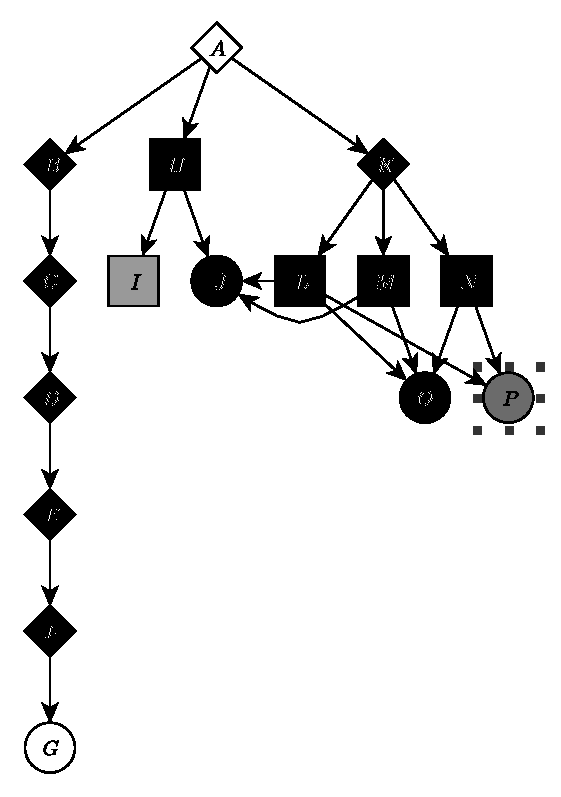
\includegraphics[scale=0.7]{images/trust-beispiel.pdf}
  \caption{Beispiel für die Berechnung der Gültigkeit von Schlüsseln}
  \label{fig:trust-beispiel}
\end{figure}

Abbildung \ref{fig:trust-beispiel} gibt ein Beispiel für die
Berechnung der Schlüsselgültigkeit unter Verwendung der
Standard-Parameter $N=1$, $M=3$ und $L=5$. Die Schlüssel $B, H$ und
$K$ wurden direkt von $A$, dem Besitzer des Schlüsselrings,
unterschrieben und sind deshalb voll gültig. Da $L, M,$ und $N$ von
$K$ unterschrieben wurden und dieser über volles Vertrauen verfügt,
sind sie ebenfalls voll gültig. $O$ sowie $J$ sind voll gültig, da sie
jeweils von drei Schlüsseln mit geringfügigem Vertrauen unterschrieben
wurden. $I$ und $P$ wurden dagegen jeweils nur von zwei Schlüsseln mit
geringfügigem Vertrauen unterschrieben und sind deshalb nicht voll
sondern nur eingeschränkt gültig. $G$ wurde zwar von einem voll
gültigen Schlüssel mit vollem Vertrauen unterschrieben. Allerdings
überschreitet die Signaturkette zu $A$ die maximale Länge von 5 und
wird deshalb nicht benutzt.

Ein öffentlicher Schlüssel, der anhand dieser Regeln nicht als
authentisch verifiziert werden kann, kann trotzdem zur Verschlüsselung
und zur Verifizierung von Signaturen verwendet werden. Allerdings
warnt GnuPG in diesem Fall vor der Verwendung.

Es muss bemerkt werden, dass keine direkte Verbindung zwischen dem
Vertrauenswert und dem G\"ultigkeitswert eines Schl\"ussels
besteht. Ein Schl\"ussel, dem voll vertraut wird, kann trotzdem
aufgrund von fehlenden Signaturketten ung\"ultig sein. Signaturen
dieses Schl\"ussels k\"onnen dann nicht benutzt werden.

\subsection{Das Keyserver-Netzwerk}
\label{sec:das-keys-netzw}

Die Verbreitung von \"offentlichen Schl\"usseln ist auf beliebigen
Wegen m\"oglich, etwa per E-Mail oder auf Webseiten. Ein zentraler
Ablageort f\"ur \"offentliche Schl\"ussel erleichtert das Auffinden
derselben aber erheblich. Im Kontext von PGP wird diese Aufgabe von
\emph{Keyservern} \"ubernommen. Dabei handelt es sich im wesentlichen
um Datenbanken von OpenPGP-Schl\"usseln, die nach verschiedenen
Kriterien (etwa nach KeyID oder UserID) durchsucht werden
k\"onnen. Benutzer k\"onnen ihre \"offentlichen auf diese Keyserver
laden, um sie der \"Offentlichkeit zur Verf\"ugung zu stellen.

Schl\"ussel k\"onnen von beliebigen Personen auf Keyserver geladen
werden, nicht nur durch die Benutzer. Auf diesem Weg werden auch
Signaturen (also Zertifikate), die durch einen Zertifizierer auf einem
Schl\"ussel angebracht wurden, verbreitet. Der Zertifizierer l\"adt
den ver\"anderten Schl\"ussel auf einen Keyserver. Dieser f\"ugt die
neuen Signaturpakete dem bisherigen Schl\"ussel hinzu. Dabei werden
stets nur Pakete zu Schl\"usseln hinzugef\"ugt, nicht \"uberschrieben
oder gel\"oscht. Auf diese Weise machen Keyserver den
Zertifikatsgraphen zug\"anglich. Selbstverst\"andlich k\"onnen
Zertifikate auch auf anderen (eventuell privaten) Wegen ausgetauscht
werden.

Um Lastverteilung und Fehlertoleranz zu erreichen, existieren mehrere
Keyserver. Diese sind als Netzwerk organisiert und synchronisieren
ihren Datenbestand st\"andig untereinander. Benutzer finden also auf
allen Keyservern des Netzwerks mit sehr geringer Verz\"ogerung den
gleichen Datenbestand\footnote{In Tests des Autoren dauerte es
  normalerweise weniger als 10 Sekunden, bis neue Schl\"ussel auf alle
  Keyserver des Verbundes propagiert waren.}. Das \"offentliche
Keyserver-Netzwerk besteht derzeit (Mai 2010) aus 48
Keyservern\cite{SKS}. Die \"ublicherweise
verwendete Keyserver-Software wird in Abschnitt
\ref{ch:Grundlagen:sec:Design:subsec:der-sks-keyserver} beschrieben.

Eine wichtige Eigenschaft des Keyserver-Netzwerks ist es, dass sich
Schl\"ussel, die einmal auf einen der dazugeh\"origen Keyserver
abgelegt wurden, nicht mehr aus dem Netzwerk entfernen lassen. Zwar
kann ein Schl\"ussel oder ein einzelnes OpenPGP-Paket aus der
Datenbank von einzelnen Keyservern gel\"oscht werden. Allerdings wird
er in diesem Fall durch die Synchronisierung mit anderen Keyservern
des Netzwerks wieder auftauchen. Das Keyserver-Netzwerk insgesamt
sieht keine Prozedur f\"ur die Entfernung von Schl\"usseln vor. Das
bedeutet, dass das \"offentliche Keyserver-Netzwerk alle\footnote{Es
  kann nicht ausgeschlossen werden, dass einzelne Schl\"ussel durch
  Softwarefehler verloren gingen. Die zahlreichen Kopien des
  Datenbestandes auf den einzelnen Keyservern und die st\"andige
  Synchronisation machen dies jedoch unwahrscheinlich.} jemals dort
ver\"offentlichten Schl\"ussel enth\"alt. Dieses Verhalten stellt
f\"ur Benutzer kein wirkliches Problem dar. Der korrekte Weg, um einen
Schl\"ussel, der aus beliebigen Gr\"unden nicht mehr benutzbar ist,
unbrauchbar zu machen, ist der Widerruf des Schl\"ussels. Umgekehrt
w\"urde eine M\"oglichkeit zur L\"oschung von Schl\"usseln einem
Angreifer die M\"oglichkeit er\"offnen, einzelne Schl\"usselteile --
beispielsweise Signaturpakete mit Widerrufssignaturen -- zu entfernen
und dadurch eigentlich widerrufene kompromittierte Schl\"ussel wieder
g\"ultig erscheinen zu lassen.

Der Widderuf eines Schl\"ussels oder einzelner Schl\"usselbestandteile
durch seinen Besitzer kann nur effektiv erfolgen, wenn die Information
\"uber den Widerruf an alle Personen verteilt wird, die den
entsprechenden \"offentlichen Schl\"ussel potentiell
benutzen. Keyserver bieten die M\"oglichkeit, die Information \"uber
den Widerruf von Schl\"usseln zentral und \"offentlich verf\"ugbar zu
machen, indem das Widerrufszertifikat auf den Keyservern verf\"ugbar
gemacht wird. Allerdings kann dieses Vorgehen nat\"urlich nur
funktionieren, wenn Benutzer ihren Schl\"usselring regelm\"assig mit
den Informationen eines Keyservers aktualisieren. Im Fall der
Kompromittierung eines Schl\"ussels ist die Information aber
zeitkritisch. Anwender sollten dann direkt informiert werden.

Indem ein Benutzer Signaturen auf einem Keyserver zur Verf\"ugung
stellt, macht er Informationen \"uber seine Beziehungen f\"ur die
\"Offentlichkeit sichtbar. In Abschnitt \ref{sec:soziale-netzwerke}
wird argumentiert, dass die Signaturbeziehungen einer Person ein
Abbild sozialer Beziehungen von unterschiedlicher Art sind. Die rein
topologische Information eines sozialen Netzwerks erlaubt detaillierte
Aussagen \"uber die Rolle einzelner Personen im
Netzwerk\cite{Carrington2005}. Benutzer m\"ussen sich daher bewusst
sein, dass die Benutzung \"offentlicher Keyserver einen Verlust von
Privatsp\"are mit sich bringt und m\"ussen dies gegen\"uber einem
m\"oglichen Gewinn an Sicherheit und Bequemlichkeit abw\"agen.

\subsection{Zustandekommen von Signaturen im Web of Trust}
\label{sec:sozi-komp-des}

\subsubsection{\"Ubliche Zertifizierungsprozeduren}
\label{sec:ubliche-zert}

Bis jetzt wurde nur erkl\"art, dass eine Signatur die
Zusicherung \"uber die Bindung eines Schl\"ussels an eine Person,
d.h. eine Identit\"at, darstellt. In diesem Abschnitt wird n\"aher
darauf eingegangen, wie solche Zusicherungen \emph{\"ublicherweise}
zustande kommen. Ausserdem werden einige Aspekte (FIXME
Rahmenbedingungen)

Bemerkt werden muss, dass der Zertifizierungsprozess im Kontext des
Web of Trust nicht formal definiert ist. Weder der OpenPGP-RFC noch
andere Standarddokumente machen dazu Vorschriften. Nur Certificate
Authorities, die PGP verwenden, und einige wenige Privatpersonen
dokumentieren ihre Verfahren zur Zertifizierung in Form von
sogenannten ``Keysigning-Policies''. Ausserdem ist dem Autor dieser
Arbeit keine Studie \"uber tats\"achlich verwendete Mechanismen
bekannt. Deshalb wird an dieser Stelle nur anekdotische Evidenz
als Eindruck von \"ublichen Praktiken pr\"asentiert.

Die Person, die eine Signatur erstellt, wird im folgenden mit
\emph{Unterzeichner}, und die Person, deren Schl\"ussel
unterschrieben wird, mit \emph{Unterzeichneter} bezeichnet. Um
die oben erw\"ahnte Zusicherung abgeben zu k\"onnen, muss der
Unterzeichner die Identit\"at des Unterzeichneten \"uberpr\"ufen und
so sicherstellen, dass sie mit der auf dem Schl\"ussel angegebenen
Identit\"at (in Form der \emph{UserID}) \"ubereinstimmt. Diese
\"Uberpr\"ufung sollte in Form eines \emph{pers\"onlichen} Treffens
stattfinden, da sonst eine sinnvolle Identit\"ats\"uberpr\"ufung im
Allgemeinen nicht m\"oglich ist. Der Unterzeichnete sollte zuerst den
Fingerabdruck seines Schl\"ussels pr\"asentieren. Anhand dieses
Fingerabdrucks kann der Unterzeichnete \"uberpr\"ufen, dass der zu
unterschreibende Schl\"ussel tats\"achlich der des Unterzeichneten
ist.  Der Unterzeichnete sollte dann ein Dokument pr\"asentieren, dass
seine Identit\"at belegt. Um die Verwendung von gef\"alschten
Dokumenten zu erschweren, wird \"ublicherweise ein amtliches
Ausweisdokument mit Lichtbild gefordert (Personalausweis,
Reisepass). Der Unterzeichner kann nun anhand des Dokumentes
\"uberpr\"ufen, dass der Unterzeichner mit der auf dem Schl\"ussel
vermerkten Identit\"at identisch ist. Damit kann der Unterzeichner den
Schl\"ussel unterschreiben und die obige Zusicherung
abgeben. Normalerweise werden beide Teilnehmer ihre Schl\"ussel
gegenseitig unterschreiben, also die Rollen von Unterzeichner und
Unterzeichnetem wechseln.

Dies sind die \"ublichen Anforderungen an einen
Zertifizierungsprozess, wie sie von ernsthaften Benutzern des Web of
Trust erwartet werden. Allerdings hindert einen Teilnehmer nichts
daran, diese Anforderungen beliebig abzuschw\"achen. Er kann
beispielsweise auf die Identit\"ats\"uberpr\"ufung von Personen
verzichten, die ihm pers\"onlich bekannt sind oder im Extremfall auf
jegliche \"Uberpr\"ufung verzichten. Allerdings ist jeder Benutzer
selbst daf\"ur verantwortlich zu entscheiden, welchen Personen er
dahingehend vertraut, korrekte Zusicherungen abzugeben.

\subsubsection{Certificate Authorities im Web of Trust}
\label{sec:cert-auth-im}

Eine Reihe von Einrichtungen agiert im Kontext des Web of Trust als
\emph{Certificate Authorities} im Sinne von Abschnitt
\ref{ch:Grundlagen:sec:PublicKeyCrypto:subsec:KeyAuth:subsubsec:PKI}. Diese
Einrichtungen bieten als Dienstleistung die Signierung von
PGP-Schl\"usseln nach \"Uberpr\"ufung der Identit\"at an. Der Prozess
bzw. die Kriterien, nach dem diese Signaturen zustande kommen, ist
dokumentiert. Dieser Prozess unterscheidet sich \"ublicherweise nicht
von dem in Abschnitt \ref{sec:ubliche-zert} beschriebenen Vorgehen.

\begin{itemize}
\item Der Heise-Verlag betreibt seit 1997 eine Certificate Authority
  im Rahmen der ``Krypto-Kampagne''. Diese hat sich zum Ziel gesetzt,
  die Verbreitung von PGP zu f\"ordern. Durch eine kostenlose
  Certificate Authority soll das Web of Trust gest\"arkt werden (FIXME
  cite).

  Die Zertifizierung wird auf Messen gegen Vorlage des
  Personalausweises angeboten. Die von dieser CA verwendeten
  Schl\"ussel haben insgesamt ca. 22000 Signaturen erstellt.
\item Die Certificate Authority CACert (FIXME link) zertifizert unter
  anderem auch OpenPGP-Schl\"ussel. Der von dieser CA verwendete
  Schl\"ussel hat ca. 3400 Schl\"ussel signiert.
\item Das Deutsche Forschungsnetzwerk (DFN) betrieb vermutlich bis zum
  Jahr 2009 eine Certificate Authority f\"ur PGP.
\end{itemize}

Das Konzept einer Certificate Authority steht nicht grunds\"atzlich im
Widerspruch zu dem des Web of Trust. Eine Verifizierungsprozedur wie
in Abschnitt \ref{sec:ubliche-zert} macht f\"ur einen Schl\"ussel
einer Certificate Authority keinen Sinn, da er \"ublicherweise nicht
mit einer einzelnen Person verbunden ist. Ein Benutzer muss
sicherstellen, dass der CA-Schl\"ussel authentisch ist und
entscheiden, ob er dem Betreiber dahingehend vertraut, die
dokumentierte Policy FIXME zuverl\"assig umzusetzen. Zus\"atzlich muss
allerdings der CA-Schl\"ussel signiert werden, um seine Signaturen
benutzen zu k\"onnen. Werden diese Signaturen auf dem CA-Schl\"ussel
ver\"offentlicht, dann ergeben sich Signaturpfade, die zu diesem
Schl\"ussel f\"uhren. Der CA-Schl\"ussel kann dann auch von
Teilnehmern, die ihn nicht direkt unterschrieben haben, als Teil ganz
normaler Signaturketten verwendet werden (sofern sie dem Betreiber der
Certificate Authority vertrauen). Certificate Authorities f\"ugen sich
also problemlos in das dezentrale Web of Trust ein.

\subsubsection{Keysigning-Parties}
\label{sec:keysigning-parties}

Das in Abschnitt \ref{sec:ubliche-zert} beschriebene \"ubliche
Verfahren betrifft zun\"achst nur zwei Personen. Wenn mehrere Personen
zusammenkommen, um ihre Schl\"ussel gegenseitig zu unterschreiben,
wird von einer \emph{Keysigning-Party} gesprochen. Die Bandbreite
dieser Veranstaltungen ist sehr gross. Sie reicht von informellen
Zusammenk\"unften mehrerer Personen, die paarweise ihre Schl\"ussel
unterschreiben, bis hin zu gr\"osseren, formalisierten Veranstaltungen
im Kontext von Konferenzen und Messen. Bei gr\"osseren Veranstaltungen
wird \"ublicherweise eine Anmeldung der Teilnehmer erwartet. F\"ur
gr\"ossere Veranstaltungen hat sich eine Reihe von ``Protokollen''
etabliert, um den Ablauf effizient zu organisieren\cite{Brennen2008}.

Gr\"ossere Keysigning-Parties Open-Source-Umfeld fanden im Jahr 2009
beispielsweise auf diesen Veranstaltungen statt:
\begin{itemize}
\item Debconf (Konferenz des Debian-Projekts) mit 113 Teilnehmern
\item FOSDEM (Open-Source-Konferenz) mit 253 Teilnehmern
\item LinuxTag (Messe) mit 132 Teilnehmern
\end{itemize}

Offensichtlich ist die Obergrenze der Signaturen, die aus einer
Keysigning-Party mit $n$ Teilnehmern entstehen k\"onnen, $n^2$. Schon
bei Veranstaltungen mit wenigen hundert Teilnehmern werden also
erhebliche Mengen von Signaturen dem Web of Trust hinzugef\"ugt.

Insbesondere auf kleinen und spontanen Veranstaltungen ist es jedem
Teilnehmer \"uberlassen, mit welchen anderen Teilnehmern er Signaturen
austauscht. \"Ublich ist allerdings, dass (fast) alle Paare von
Teilnehmern Signaturen austauschen. Ein hervorstechendes Merkmal
vieler Keysigning-Parties ist also eine (fast) vollst\"andige
Vernetzung ihrer Teilnehmer.

\subsubsection{PGP im Debian-Projekt}
\label{sec:foobar-fixme}

In einer Reihe von Open-Source-Projekten spielen PGP und das Web of
Trust eine wichtige Rolle. Im Debian-Projekt beispielweise werden
PGP-Schl\"ussel unter anderem benutzt, um alle bereitgestellten
Softwarepakete durch den zust\"andigen Entwickler signieren zu
lassen. Auf diese Weise wird \"uberpr\"uft, dass ein hochgeladenes
Paket tats\"achlich von dem verantwortlichen Projektmitglied stammt
und nicht ver\"andert wurde. Dazu muss jeder etwa 1000
Debian-Entwickler \"uber einen Schl\"ussel verf\"ugen, der von
mindestens einem anderen Debian-Entwickler verifiziert und
unterschrieben wurde. Auf diese Weise bildet sich bereits innerhalb
des Projekts ein Web of Trust, dass einen Teil des globalen Web of
Trust darstellt. PGP scheint eine wichtige Rolle in der Kultur des
Projekts zu spielen. Darauf weist beispielsweise hin, dass auf Treffen
von Projektmitgliedern oft Keysigning-Parties abgehalten werden, um
das Web of Trust zu st\"arken. Ausserdem signiert eine
\"uberdurchschnittliche Anzahl von Debian-Entwicklern ihre E-Mails auf
projektinternen Mailinglisten.

\section{Graphentheorie und Netzwerkanalyse}
\label{sec:graph-und-netzw}

\subsection{Graphentheorie allgemein}
\label{ch:Grundlagen:sec:Graphentheorie}

Dieser Abschnitt f\"uhrt einige grundlegende graphentheroretische
Begriffe nach \cite{Brandes2004} ein.
  
Ein \emph{Netzwerk} bezeichnet eine Ansammlung von Objekten, zwischen
denen bilaterale Beziehungen bestehen. Das hier betrachtete Netzwerk
besteht aus einer Ansammlung von OpenPGP-Schl\"usseln, zwischen denen
Beziehungen in Form von Signaturen bestehen. Ein Netzwerk kann durch einen
Graphen repr\"asentiert werden.

Ein \emph{Graph} $G=(V, E)$ besteht aus einer endlichen Menge $V$ von
\emph{Knoten} und einer endlichen Menge $E$ von \emph{Kanten}, die je
zwei Knoten miteinander verbinden. Die Anzahl $|V|$ der Knoten wird mit
$n$ und die Anzahl der Kanten mit $m$ bezeichnet. Zwei durch eine
Kante verbundene, \emph{benachbarte} Knoten heissen
\emph{adjazent}. In einem \emph{ungerichteten} Graphen ist $E$ eine
Teilmenge von $V\times V$, also eine Menge von Kanten $\{u, v\}$, die
zwei Knoten $u \in V$ und $v\in V$ verbinden. In einem
\emph{gerichteten} Graphen besteht eine Kante aus einem geordneten
Paar $(u, v)$ von Knoten. Eine gerichtete Kante $(u, v)$ f\"uhrt vom
\emph{Ursprung} $u$ zum \emph{Ziel} $v$.

Ein Graph ist \emph{vollst\"andig}, wenn er alle m\"oglichen Kanten
enth\"alt.

Der \emph{Grad} $d(v)$ eines Knotens $v$ in einem ungerichteten
Graphen bezeichnet die Anzahl der Kanten, die diesen Knoten
enthalten. Die \emph{Nachbarschaft} $N(v)$ bezeichnet die Menge der
Knoten, die zu $v$ adjazent sind. In einem gerichteten Graphen
bezeichnet der \emph{eingehende Grad} $d^{-}(v)$ die Anzahl der
Kanten, die den Knoten $v$ als Ziel enthalten, und der
\emph{ausgehende Grad} $d^{+}(v)$ die Anzahl der Kanten, die $v$ als
Ursprung enthalten.

Ein \emph{Kantenzug} zwischen Knoten $v_0$ und $v_k$ in einem Graphen
$G=(V, E)$ ist eine alternierende Folge $(v_0, e_1, v_1, e_2, \dots,
v_{k-1}, e_k, v_k)$, wobei $v_i \in V$, $e_i \in E$, sowie $e_i =
\{v_{i-1}, v_{i}\}$ in einem ungerichteten Graphen bzw. $e_i =
(v_{i-1}, v_{i})$ in einem gerichteten Graphen. Der Kantenzug hat die
\emph{L\"ange} $i$. Ein Kantenzug heisst \emph{einfach}, wenn $e_i \ne
e_j$ f\"ur $i \ne j$ gilt.  Ein einfacher Kantenzug heisst
\emph{Pfad}, wenn $v_0, \dots, v_k$ paarweise verschieden sind. Die
\emph{Distanz} $d(u, v)$ von einem Knoten $u$ zu einem Knoten $v$ ist die
L\"ange eines k\"urzesten Pfades zwischen $u$ und $v$. Besteht kein
Pfad von $u$ nach $v$, so wird $d(u,v) = \infty$ definiert.

Ein Graph $G' = (V', E')$ ist ein \emph{Teilgraph} eines Graphen $G =
(V, E)$, wenn $E' \subseteq E$ und $V' \subseteq V$ gelten. Ein
Teilgraph $G' = (V', E')$ eines Graphen $G$ ist durch eine eine
Knotenmenge $V'$ \emph{induziert}, wenn $E' = \{(u, v) : u \in V, v
\in V, (u, v) \in E\}$ gilt.

Eine \emph{Partitionierung} oder \emph{Zerlegung} eines Graphen
bezeichnet Mengen $V_1, \dots, V_n$ mit $V_i \cap V_j = \emptyset
\quad \forall 1 \le i, j \le n$ und $V_1 \cup \dots \cup V_n = V$.

Ein ungerichteter Graph heisst \emph{zusammenh\"angend}, wenn es
zwischen allen Knotenpaaren $u, v$ einen Pfad gibt. Eine
\emph{Zusammenhangskomponente} eines Graphen $G$ ist ein
\emph{maximaler}, zusammenh\"angender induzierter Teilgraph von
$G$. Ein gerichteter Graph ist \emph{stark zusammenh\"angend}, wenn es
f\"ur jeden Knoten einen gerichteten Pfad zu jedem anderen Knoten gibt. Eine
\emph{starke Zusammenhangskomponente} eines Graphen $G$ ist dann ein
maximaler, stark zusammenh\"angender induzierter Teilgraph von $G$.

\subsection{Netzwerkstatistiken}
\label{ch:Grundlagen:sec:Netzwerkanalyse:subsec:Statistiken}

In diesem Abschnitt werden einige Kennzahlen nach
\cite{Brinkmeier2004} definiert, die die Struktur eines Graphen
charakterisieren.

Die Distanz zwischen zwei Knoten wurde bereits im vorherigen Abschnitt
definiert. Ausgehend davon k\"onnen die Distanzen \emph{eines Knotens}
durch die durchschnittliche Distanz dieses Knotens zu allen anderen
Knoten charakterisiert werden:

\begin{equation}
  \label{eq:1}
  \bar{d}(u) = \frac{1}{n-1} \sum_{v \ne u} d(u, v)
\end{equation}

F\"ur einen gesamten Graphen gibt die \emph{charakteristische oder
  durchschnittliche Distanz} den Durchschnitt aller Distanzen in
diesem Graphen an:

\begin{equation}
  \label{eq:2}
  \bar{d} = \frac{1}{n^2 - n} \sum_{u \ne v \in V} d(u, v)
\end{equation}

Die \emph{Eccentricity} eines Knotens $u$ ist definiert als die
maximale Distanz zu einem anderen Knoten, also

\begin{equation}
  \label{eq:3}
  \epsilon(u) = \max\{d(u,v) | v \in V\}
\end{equation}

Davon ausgehend  wird der \emph{Durchmesser} eines Graphen als Maximum
und der Radius als Minimum \"uber die Eccentricity aller Knoten
definiert. Durchmesser und Radius geben also die Ober-
bzw. Untergrenze der Pfadl\"ange an, mit der ein Knoten alle anderen
Knoten erreichen kann. Bemerkt werden muss, dass alle auf Distanzen
basierenden Kennzahlen im Falle eines nicht (stark)
zusammenh\"angenden Graphen unendlich sind. Dieses Problem wird im
weiteren vermieden, indem diese Kennzahlen nur f\"ur (starke)
Zusammenhangskomponenten berechnet werden.

Als Verallgemeinerung der Nachbarschaft eines Knotens wird die
\emph{h-Nachbarschaft} eines Knotens als
\begin{equation}
  \label{eq:4}
  N_h(v) = \{ u \in V | d(v, u) \le h \}
\end{equation}
definiert, d.h. die Menge der Knoten, zu denen die Distanz von $v$ aus
h\"ochstens $h$ betr\"agt.

Der \emph{Clustering-Koeffizient} nach Watts und Strogatz ist ein Mass
daf\"ur, wie \emph{transitiv} die Beziehungen in einem Netzwerk
sind. Ein hoher Clustering-Koeffizient steht f\"ur eine hohe
Wahrscheinlichkeit, dass zwei Nachbarn $v$ und $w$ eines Knotens $u$
auch untereinander verbunden sind. Sei $G = (V, E)$ ein ungerichteter
Graph. Ein Dreieck $\bigtriangleup = \{V_{\bigtriangleup},
E_{\bigtriangleup}\}$ ist ein vollst\"andiger Teilgraph der Gr\"osse 3
von $G$. Die Anzahl der Dreiecke \emph{eines Knotens} wird mit
$\lambda(v) = |\{\bigtriangleup : v \in V_{\bigtriangleup}\}|$
bezeichnet. Ein \emph{Tripel} an einem Knoten $v$ ist ein Teilgraph
von $G$ bestehend aus 2 Kanten sowie $v$ und 2 weiteren Knoten, so
dass beide Kanten $v$ enthalten. Die Anzahl der Tripel eines Knotens
$v$ kann durch den Grad $d(v)$ ausgedr\"uckt werden als
$\tau(v)=\binom{d(v)}{2}$. Der \emph{lokale} Clustering-Koeffizient
$c_v$ eines Knotens wird dann als
\begin{equation}
  \label{eq:5}
  c(v) = \frac{\lambda(v)}{\tau(v)}
\end{equation}
definiert. $c(v)$ gibt also gewissermassen an, wie viele der
m\"oglichen Dreiecke an $v$ auch tats\"achlich Dreiecke sind. Der
globale Clustering-Koeffizient von $G$ ist dann
\begin{equation}
  \label{eq:6}
  C(G) = \frac{1}{|V'|} \sum_{v \in V'}c(v)
\end{equation}
wobei $V' = \{v \in V : d(v) \ge 2\}$ gesetzt wird, um nicht
definierte Werte f\"ur $\tau(v)$ zu vermeiden.

Die \emph{Transitivity} nach Newman et al. dr\"uckt zwar den gleichen
Sachverhalt aus wie der in dieser Arbeit verwendete
Clustering-Koeffizient, ist aber nicht \"aquivalent zu diesem und
sollte nicht verwechselt werden.

knn

\begin{equation}
  \label{eq:9}
  <knn> = \sum_{k'} k'P_c (k'|k)
\end{equation}

Ein verwandtes Mass wird von Newman eingef\"uhrt: Ein Netzwerk zeigt
\emph{assortative mixing}, wenn Knoten mit hohem Grad haupts\"achlich
mit solchen Knoten verbunden sind, die ebenfalls einen hohen Grad
haben\cite{PhysRevLett.89.208701}. Diese Eigenschaft wird durch den
\emph{Assortativity-Koeffizienten} (ebd.)  gemessen, dessen Werte
zwischen -1 und 1 liegen. Positive Werte f\"ur ein Netzwerk zeigen
assortative mixing an, bei negativen Werten zeigt das Netzwerk kein
assortative mixing. Newman gibt an, dass assortative mixing eine
Eigenschaft ist, die viele soziale Netzwerke von anderen Netzwerken --
etwa technologischer oder biologischer Natur unterscheidet. Die
meisten sozialen Netzwerke zeigen assortative mixing, w\"arend die
restlichen dies nicht tun.

\subsection{Soziale Netzwerke}
\label{sec:soziale-netzwerke}

Ein \emph{soziales Netzwerk} ist nach Newman\cite{newman:167} eine
Menge von Personen bzw. Gruppen von Personen, zwischen denen
Beziehungen bzw. Kontakte bestehen. Die Art dieser Interaktionen ist
dabei beliebig: Soziale Netzwerke, die in der Literatur analysiert
wurden, beinhalten Freundschaftsnetzwerke von Schulkindern, Netzwerke
von sexuellen Kontakten und Netzwerke von Gesch\"aftsbeziehungen
(ebd.).

Die im Web of Trust vorhandenen Schl\"ussel k\"onnen als
Repr\"asentationen der Besitzer dieser Schl\"ussel gedacht
werden. Allerdings ist dies keine Eins-zu-eins-Beziehung, da eine
Person \"uber beliebig viele Schl\"ussel verf\"ugen kann. Die
Beziehung dieser Personen im Web of Trust repr\"asentiert zun\"achst
nur eine Signatur, also eine Zusicherung \"uber die Bindung zwischen
dem signierten Schl\"ussel und der Identit\"at des Besitzers. Es
scheint allerdings recht unwahrscheinlich, dass solche Signaturen
zwischen Personen entstehen, die sich v\"ollig unbekannt sind und in
keiner Beziehung zueinander stehen. Stattdessen wird in dieser Arbeit
davon ausgegangen, dass sich Signaturen in den meisten F\"allen anhand
von bereits bestehenden sozialen Kontakten zwischen den Besitzern der
Schl\"ussel ergeben\cite{Capkun2002}. Das Sprektum m\"oglicher
Beziehungen ist dabei nat\"urlich sehr weit und umfasst mindestens
alle Gruppen von Personen, die potentiell ein Interesse an
vertraulicher und authentifizierter E-Mail-Kommunikation haben: Es
kann sich dabei um pers\"onliche Bekanntschaften handeln, also etwa um
Freunde und Bekannte. Genauso kann sich die Beziehung auch prim\"ar
durch die Mitgliedschaft in einer gemeinsamen Gruppe oder Institution
ergeben. Denkbar sind hier zum Beispiel Beziehungen, die sich aus
Arbeitsverh\"altnissen oder einer Ausbildung ergeben, also Unternehmen
oder akademische Einrichtungen. Genausogut kann es sich aber um die
Mitgliedschaft in einem Open-Source-Projekt, einem Verein oder einer
politischen Organisation handeln. Auch Zusammenh\"ange, die nicht
\"uber eine formale Mitgliedschaft in einer festen Gruppierung
entstehen, sind m\"oglich.

Zumindest im Fall von gr\"osseren, formalen Keysigning-Parties scheint
zun\"achst nicht notwendigerweise eine Verbindung zwischen den
Teilnehmern (abgesehen von der Teilnahme selbst) zu bestehen. Es ist
aber auch der Kontext relevant, in dem die Keysigning-Party
stattfindet. Bei einer Konferenz oder Messe kann es sich um ein
Ereignis mit einer klar definierten Zielgruppe handeln, die wiederum
einer Gruppe zuordnenbar ist (z.B. im Fall der
``Debconf''-Konferenzen). Ist dies nicht m\"oglich, so handelt es sich
immerhin um eine Gruppe von Personen, die \"uber ein gemeinsames
Interessengebiet verf\"ugen (beispielsweise im Fall der
``LinuxTag''-Keysigning-Parties).

\subsection{Small-World-Effekt}
\label{sec:small-world-effekt}

Milgram f\"uhrte ein Experiment durch, bei dem Briefe von Person zu
Person\footnote{Teilnehmer wurden aufgefordert, die Briefe an ihnen
  direkt bekannte Personen weiterzugegen, von denen sie annahmen, dass
  sie sich ``n\"aher'' am Ziel befinden w\"urden.} weitergegeben
wurden, um sie von zuf\"allig ausgew\"ahlten Absendern zu ebenfalls
zuf\"allig ausgew\"ahlten, geographisch weit entfernten Empf\"angern
zu transportieren\cite{Travers1969}. Diese Briefe erreichten ihr Ziel
im Durchschnitt \"uber nur sechs Zwischenstationen\footnote{71\% der
  Briefe erreichten ihr Ziel nicht.}. Mit diesem Experiment wurde
gezeigt, dass Paare von Akteuren in einem sozialen Netzwerk nur durch
wenige ``Zwischenschritte'' miteinander verbunden sind. Das Ph\"anomen
``kleiner'' durchschnittlicher Pfadl\"angen wird als
\emph{Small-World-Effekt} bezeichnet. Die meisten Netzwerke aus der
realen Welt -- insbesondere soziale Netzwerke -- scheinen diesen
Effekt aufzuweisen\cite{newman:167}. Eine pr\"azisere Formulierung
ist, dass die durchschnittliche Distanz nur logarithmisch mit der
Anzahl der Knoten w\"achst.

Auch zuf\"allige Graphen verf\"ugen \"uber eine geringe
durchschnittliche Distanz. Strogatz und Watts bemerken, dass viele
reale Netzwerke zus\"atzlich \"uber ausgepr\"agtes Clustering
verf\"ugen, also \"uber einen hohen
Clustering-Koeffizienten\cite{Watts1998}.

\subsection{Skalenfreie Netzwerke}
\label{sec:skal-netzw}

Definition einer Power-Law-Verteilung. Verbindung mit Netzwerken:
Power-Law in Gradverteilung. Barabasi: Skale free. Netzwerke mit
dieser Eigenschaft \"uberall gefunden (bsp: sozial, biologisch,
technisch). allerdings f\"ur viele dieser netzwerke bestritten, dass
es sich um ein wirkliches power-law handelt und dass
preferential-attachment als erzeugungsmechanismus wirkt. Erzeugendes
Modell vorgeschlagen, dass Graphen mit Power-law-Verteilung erzeugt ->
preferential attachment.

welche eigenschaften werden scale-free networks zugeschrieben? li et
al. bemerken, dass konfusion herrscht, welche eigenschaften
skalenfreie netzwerke ausmachen und welche daraus folgen. vielleicht
auch biologen-essay zitieren.

\cite{Barabasi1999} 
baz

\subsection{Communities}
\label{ch:Grundlagen:sec:Netzwerkanalyse:subsec:Communities}

Dieser Abschnitt f\"uhrt den Begriff der \emph{Community} ein,
definiert das G\"utemass \emph{Modularity} und beschreibt einige
Algorithmen zur Erkennung von Communities in Netzwerken. Sofern nicht
anders angegeben, wurde als Quelle ein \"Ubersichtsartikel von
Fortunato \cite{Fortunato2010} benuzt.

\subsubsection{Grundlegende Begriffe}
\label{sec:grundl-begr}

In vielen -- insbesondere sozialen -- Netzwerken neigen die Teilnehmer
dazu, \emph{Gruppen} zu bilden. In sozialen Netzwerken bilden sich
etwa Gruppen von Teilnehmern, die \"uber famili\"are,
freundschaftliche oder professionelle Beziehungen miteinander
verbunden sind. Ein besonders intensiv untersuchter Typ solcher
Netzwerke entsteht aus Kooperations- oder Koautornetzwerken von
Wissenschaftlern, in denen sich Wissenschaftler nach ihren
Fachgebieten gruppieren. Andere Beispiele von Netzwerken, in denen
Gruppenbildung stattfindet, sind Netzwerke aus der Biologie,
beispielweise Netzwerke von Protein-Protein-Interaktionen, in denen
sich funktionell \"ahnliche Proteine gruppieren, die an den gleichen
biologischen Prozessen teilnehmen. Das hier zentrale Merkmal dieser
Gruppen oder \emph{Communities} ist die Tatsache, dass Mitglieder
einer Gruppe normalerweise deutlich mehr Beziehungen zu anderen
Mitgliedern dieser Gruppe haben als zu Teilnehmern ausserhalb. Eine
solche Community sollte sich also auch in der Struktur des Graphen
wieder finden, der das Netzwerk beschreibt. In der Tat teilen viele --
insbesondere die oben angef\"uhrten -- Beispiele von Netzwerken die
Eigenschaft, dass die Kanten des Netzwerks nicht gleichm\"assig
verteilt sind. Stattdessen finden sich Gruppen von Knoten, in denen
eine hohe Dichte von Kanten herrscht, w\"ahrend zwischen diesen
Gruppen nur wenige Kanten bestehen.

In der Literatur scheint keine strenge Definition einer Community zu
existieren, die allgemein akzeptiert ist. Stattdessen wird ein
intuitives Verst\"andis verwendet, nach dem Communities \emph{dichte}
Teilbereiche eines Graphen sind, also Gruppen von Knoten, die
untereinander ``viele'' Kanten haben, w\"arend zu nicht in der Gruppe
liegenden Knoten nur ``wenige'' Kanten bestehen.

Da ein Graph \"uber ein konkretes Netzwerk abstrahiert und nur noch
die Struktur abbildet, werden auch bei der Community-Erkennung nur
Informationen benutzt, die in der Topologie des Graphen kodiert sind. 

\cite{Girvan2002}

\subsubsection{Modularity}
\label{sec:modularity}

Eine solche hierarchische Zerlegung macht noch keine Aussage
dar\"uber, wie gut die Zerlegung auf einer bestimmten Ebene die
tats\"achliche Community-Struktur wiedergibt. Um diese Frage zu
beantworten, wurde ebenfalls von Newman als Mass f\"ur die Qualit\"at
einer Zerlegung die sogenannte \emph{Modularity} definiert. Gegeben
einen ungerichteten Graphen $G=(V, E)$ und eine Zerlegung dieses
Graphen $\mathcal{C} = C_1, ..., C_n$ wird die Modularity $Q$
definiert als
\begin{equation}
  \label{eq:modularity}
  Q =
  \frac{1}{2m}\sum_{u, v \in V}\left(A_{uv}-\frac{d_id_j}{2m}\right)\delta(C_u, C_v)
\end{equation}

\subsubsection{Weitere Algorithmen}
\label{sec:algorithmen}

Seit der Arbeit von Newman wurde eine Vielzahl weiterer Methoden zur
Erkennung von Communities vorgestellt. An dieser Stelle werden 3
Methoden n\"aher beschrieben, die in dieser Arbeit verwendet
werden. Einen Gesamt\"uberblick bietet ein \"Ubersichtsartikel von
Fortunato \cite{Fortunato2010}.

\paragraph{Algorithmus von Blondel et al.}
\label{sec:algor-von-blond}

\paragraph{COPRA}
\label{sec:copra}

%% ==============================
\section{Verwandte Arbeiten}
%% ==============================
\label{ch:Grundlagen:sec:RelatedWork}

An dieser Stelle wird nur auf Arbeiten eingegangen, die sich mit der
Netzwerkstruktur des Web of Trust bei PGP besch\"aftigen. F\"ur einen
\"Uberblick \"uber Arbeiten zur Struktur von anderen Netzwerken sei
auf \cite{newman:167}und f\"ur Arbeiten zur Community-Struktur von
anderen Netzwerken auf \cite{Fortunato2010} verwiesen.

Capkun et al. \cite{Capkun2002} untersuchten strukturelle Aspekte der
gr\"ossten starken Zusammenhangskomponente eines PGP-Netzwerkes aus
dem Jahr 2001. Dieses Netzwerk zeigte eine geringe charakteristische
Distanz und einen hohen Clustering-Koeffizient. Ausserdem stimmte die
Verteilung der aus- und eingehenden Grade mit einem Power-Law
\"uberein. Die Autoren argumentieren, dass Netzwerke, die aus
Zertifikatsbeziehungen entstehen, naturgem\"ass den Small-World-Effekt
zeigen, da sich die Zertifikate anhand schon bestehender
Vertrauensbeziehungen ergeben. Die Autoren geben ausserdem noch ein
Netzwerkmodell an, dass Graphen erzeugen soll, die in den
beschriebenen Charakteristiken dem PGP-Netzwerk \"ahneln.

Arenas et al. \cite{Boguna2004} analysierten ein PGP-Netzwerk aus dem
gleichen Jahr. Das Netzwerk wurde von vornherein in ein ungerichtetes
Netzwerk umgewandelt, indem nicht gegenseitige Kanten entfernt
wurden. Sie betrachteten die Gradverteilung, den
Clustering-Koeffizienten und die Korrelation von Graden benachbarter
Knoten. Dabei folgt die Verteilung der Knotengrade einem Power-Law mit
einem exponentiellen Cutoff FIXME. Der Clustering-Koeffizient des
Netzwerkes betr\"agt $C=0.4$, ist also recht hoch. Die Grade
benachbarter Knoten sind positiv korreliert. Ausserdem benutzten die
Autoren den in Abschnitt \ref{sec:grundl-begr}erw\"ahnten Algorithmus
von Girvan und Newman, um eine Community-Zerlegung des Netzwerks zu
berechnen. Die Verteilung der Gr\"osse dieser Communities folgt wieder
einem Power-Law.

Neben diesen akademischen Arbeiten gibt es mehrere Ans\"atze aus der
PGP-Community, die Netzwerkstruktur zu untersuchen. Das
Wotsap-Projekt\cite{Cederlof} stellt einen t\"aglich aktualisierten
Datensatz bereit, der die Vernetzungsstruktur der gr\"ossten starken
Zusammenhangskomponente des Web of Trust darstellt. Diese Daten werden
werden f\"ur eine Webapplikation benutzt, die k\"urzeste Pfade
zwischen Schl\"usseln berechnet und visualisiert und so bei der
Nutzung von Zertifikatspfaden behilflich sein soll. In Abschnitt
\ref{ch:Grundlagen:sec:WarumEigene} wird der Wotsap-Datensatz n\"aher
betrachtet und begr\"undet, warum er in dieser Arbeit nicht verwendet
wurde. 

Henk P. Penning berechnet anhand der Wotsap-Daten regelm\"assig
strukturelle Eigenschaften des Web of Trust bzw. von dessen gr\"osster
starker Zusammenhangskomponente \cite{Penning}. Dies beinhaltet die
Entwicklung der Gr\"osse dieser Komponente und der durchschnittlichen
Distanzen \"uber die Zeit, die Verteilung der Knotengrade und die
Verteilung durchschnittlicher Distanzen pro Knoten. Ausserdem wird die
Robustheit des Netzwerkes bei der Entfernung von zuf\"allig
ausgew\"ahlten bzw. besonders gut vernetzten Knoten simuliert.

%%% Local Variables: 
%%% mode: latex
%%% TeX-master: "diplarb"
%%% End: 
